\documentclass{article}
\usepackage[utf8]{inputenc}

\newcommand{\nirpdftitle}{The Sato--Tate Conjecture}
\usepackage{import}
\inputfrom{../../notes}{nir}
\usepackage[backend=biber,
    style=alphabetic,
    sorting=ynt
]{biblatex}
\setcounter{tocdepth}{2}

\pagestyle{contentpage}

\title{The Sato--Tate Conjecture}
\author{Nir Elber}
\date{Fall 2024}
\usepackage{graphicx}

\begin{document}

\maketitle

\begin{abstract}
	This is an expository note for two talks on the Sato--Tate conjecture. In the first talk, we will state the Sato--Tate conjecture for abelian varieties. In the second talk, we will discuss some results related to Sato--Tate groups of the so-called Fermat curves $y^p=x^a(x-1)$, where $p$ is prime and $a\in\{1,2,\ldots,p-1\}$.
\end{abstract}

\tableofcontents

\section{Stating the Sato--Tate Conjecture}
In this first talk, we will work our way towards stating the Sato--Tate conjecture for abelian varieties. We will gradually increase the amount of assumed background.

\subsection{Quadratic Equations}
In order to get a dishonest taste for the sort of results we are after, we will begin with the case of quadratic equations. Fix a monic quadratic polynomial $f(x)=x^2+ax+b$ with nonzero discriminant $a^2-4b$, and consider the curve
\[C\colon y^2=f(x).\]
Technically speaking, we understand $C_f$ to cut out a smooth projective curve in $\PP^2_\QQ$ given by homogenizing.
\begin{example}
	For this section, it will be enough to follow the example $C\colon y^2=x^2+1$ around. The polynomial $x^2+1$ has discriminant $-4$.
\end{example}
Because this is a talk about arithmetic geometry, we are interested in the number of points on $C_f$. Studying points over $\QQ$ or $\ZZ$ is rather difficult (and will continue to get harder when we change the curve later), so we will content ourselves with studying the number of points over finite fields. Even though our curve is a priori defined over $\QQ$, we see that $f(x)\in\ZZ[x]$ allows us to give $C_f$ a model over $\ZZ$ given by the same equation. In this way, we can formally make sense of $C(\FF_q)$ for any finite field $\FF_q$.
\begin{remark}
	In practice, one can think about $C(\FF_q)$ as the number of pairs $(x,y)\in\FF_q^2$ satisfying the equation given by $C$. The above process of finding an integral model should be thought of as some formal general procedure.
\end{remark}
\begin{remark}
	Our choice of integral model may not always make sense at all primes $p$. Notably, we would like for $C_f$ to define a smooth curve over $\FF_p$, but this requires $a^2-4b\ne0$ (for example). (For odd primes $p$, smoothness is equivalent to $a^2-4b\ne0$.) Over $\QQ$, this was a hypothesis, but in general, $a^2-4b$ can vanish$\pmod p$ for some primes $p$. For example, $y^2=x^2+1$ fails to be smooth over $\FF_2$.
\end{remark}
Let us begin with an expectation for $C(\FF_q)$. For each $x\in\FF_q$, it will be difficult to control the value of $f(x)$. However, about half of $\FF_q$ has two square roots, and about half of $\FF_q$ has no square roots, so it seems reasonably to expect that each $f(x)\in\FF_q$ has on average one square root. Thus, we may expect that
\[C(\FF_q)\approx q+1,\]
where we have added $1$ to include the point(s) at infinity. Let's see what we get.
\begin{example}
	We continue with the curve $C\colon y^2=x^2+1$. A computer program gives the following output.
	\[\begin{array}{c|ccccccccccccccccc}
		p & 3 & 5 & 7 & 11 & 13 & 17 & 19 & 23 & 29 & 31 & 37 & 41 & 43 & 47 \\\hline
		\#C(\mathbb F_p) & 4 & 6 & 8 & 12 & 14 & 18 & 20 & 24 & 30 & 32 & 38 & 42 & 44 & 48 \\
		p+1 & 4 & 6 & 8 & 12 & 14 & 18 & 20 & 24 & 30 & 32 & 38 & 42 & 44 & 48
	\end{array}\]
\end{example}
Huh, it looks like our guess was pretty spot-on.
\begin{exe}
	For a curve $C\colon y^2=x^2+d$ for some $d\in\ZZ$, show that $\#C(\FF_q)=q+1$ for any finite field $\FF_q$. You may find it helpful to use the substitution $(s,d)=(x+y,x-y)$.
\end{exe}
\begin{remark}
	Intuitively, what is going on here is that quadratics cut out genus $0$ curves, which must all be isomorphic to $\PP^1$.
\end{remark}

\subsection{Two Elliptic Curves}
Let's move on to a more nontrivial example. Most of this first talk will be interested in elliptic curves, for which we pick up the following concrete definition.
\begin{definition}[elliptic curve]
	Fix a field $K$ of characteristic not equal to $2$ or $3$. Then an \textit{elliptic curve} is a curve of the form
	\[E\colon y^2=x^3+ax+b,\]
	where $a,b\in K$, and the discriminant $-4a^3-27b^2$ is nonzero. As usual, $E$ is understood to cut out a smooth projective curve in $\PP^2_K$ given by homogeneizing to $Y^2Z=X^3+aXZ^2+bZ^3$, so there is one point $[0:1:0]$ at infinity.
\end{definition}
For today, all of our elliptic curves $E$ will be defined over $\QQ$ and pretty good integral models.
\begin{example} \label{ex:ec-as-c-mod-lattice}
	For any lattice $\Lambda\subseteq\CC$, it turns out that one can realize $\CC/\Lambda$ as an elliptic curve over $\CC$.
\end{example}
\begin{example}
	We will follow around the two elliptic curves
	\[E_1\colon y^2=x^3+1\qquad\text{and}\qquad E_2\colon y^2=x^3+x+1\]
	for this section. Though they look similar, these two curves have very different behavior!
\end{example}
As in the previous section, we note that one can frequently define a notion of $E(\FF_q)$. Namely, the cubic equation defining $E$ will only have finitely many denominators, and the discriminant of the cubic equation will only have finitely many prime factors; away from these primes, the equation defining $E$ will define a perfectly reasonable elliptic curve over $\FF_{p^r}$ for any $r\ge1$.
\begin{example}
	We discuss models for our elliptic curves $E_1$ and $E_2$. Note that their defining equations have no denominators.
	\begin{itemize}
		\item We see that $E_1\colon y^2=x^3+1$ has discriminat $-27$, so we get an elliptic curve over $\FF_{p^r}$ for any $p\ne3$.
		\item Similarly, the curve $E_2\colon y^2=x^3+x+1$ has discriminant $-31$, so we get an elliptic curve over $\FF_{p^r}$ for any $p\ne31$.
	\end{itemize}
\end{example}
Once again, for any value of $x$, there is no reason to expect $x^3+ax+b$ to be a square or not, so a reasonable expectation is for
\[E(\FF_q)\approx q+1.\]
Let's see what we get.
\begin{example}
	We continue with the two elliptic curves $E_1\colon y^2=x^3+1$ and $E_2\colon y^2=x^3+x+1$.
	\[\begin{array}{c|ccccccccccccccccc}
		p & 5 & 7 & 11 & 13 & 17 & 19 & 23 & 29 & 37 & 41 & 43 & 47 \\\hline
		\#E_1(\mathbb F_p) & 6 & 12 & 12 & 12 & 18 & 12 & 24 & 30 & 48 & 42 & 36 & 48 \\
		\#E_2(\mathbb F_p) & 9 & 5 & 14 & 18 & 18 & 21 & 28 & 36 & 48 & 35 & 34 & 60 \\
		p+1 & 6 & 8 & 12 & 14 & 18 & 20 & 24 & 30 & 38 & 42 & 44 & 48
	\end{array}\]
\end{example}
Our guess seems to be pretty close but not quite spot-on. Let's examine the error.
\begin{example}
	We continue with the two elliptic curves $E_1\colon y^2=x^3+1$ and $E_2\colon y^2=x^3+x+1$.
	\[\begin{array}{c|ccccccccccccccccc}
		p & 5 & 7 & 11 & 13 & 17 & 19 & 23 & 29 & 37 & 41 & 43 & 47 \\\hline
		\#E_1(\mathbb F_p)-(p+1) & 0 & 4 & 0 & -2 & 0 & -8 & 0 & 0 & 10 & 0 & -8 & 0 \\
		\#E_2(\mathbb F_p)-(p+1) & 3 & -3 & 2 & 4 & 0 & 1 & 4 & 6 & 10 & -7 & -10 & 12
	\end{array}\]
\end{example}
The error seems to be small, but perhaps it is difficult to quantify. We now state a theorem.
\begin{theorem}[Hasse--Weil] \label{thm:hasse-weil}
	Fix an elliptic curve $E$ defined over a finite field $\FF_q$. Then
	\[\left|\#E(\FF_q)-(q+1)\right|\le2\sqrt q.\]
\end{theorem}
We will not prove this, but we will state a more general version later. For now, we will content ourselves with the following example.
\begin{example}
	We continue with the two elliptic curves $E_1\colon y^2=x^3+1$ and $E_2\colon y^2=x^3+x+1$.
	\[\begin{array}{c|ccccccccccccccccc}
		p & 5 & 7 & 11 & 13 & 17 & 19 & 23 & 29 & 37 & 41 & 43 & 47 \\\hline
		E_1(\mathbb F_p)-(p+1) & 0 & 4 & 0 & -2 & 0 & -8 & 0 & 0 & 10 & 0 & -8 & 0 \\
		E_2(\mathbb F_p)-(p+1) & 3 & -3 & 2 & 4 & 0 & 1 & 4 & 6 & 10 & -7 & -10 & 12 \\
		\floor{2\sqrt{p}} & 4 & 5 & 6 & 7 & 8 & 8 & 9 & 10 & 12 & 12 & 13 & 13
	\end{array}\]
\end{example}
The bound seems to hold and even come close to equality quite frequently! This motivates us to define
\[a_q(E)\coloneqq\frac{\#E(\FF_q)-(q+1)}{\sqrt q}\in[-2,2].\]
Here is the table again.
\begin{example}
	We continue with the two elliptic curves $E_1\colon y^2=x^3+1$ and $E_2\colon y^2=x^3+x+1$.
	\[\begin{array}{c|ccccccccccccccccc}
		p & 5 & 7 & 11 & 13 & 17 & 19 & 23 & 29 & 37 & 41 & 43 & 47 \\\hline
		a_p(E_1) & 0.00 & 1.51 & 0.00 & -0.56 & 0.00 & -1.84 & 0.00 & 0.00 & 1.64 & 0.00 & -1.22 & 0.00 \\
		a_p(E_2) & 1.34 & -1.13 & 0.60 & 1.11 & 0.00 & 0.23 & 0.83 & 1.11 & 1.64 & -1.09 & -1.53 & 1.75
	\end{array}\]
\end{example}
These numbers appear sufficiently random (aside from maybe the large number of $0$s), so we can state a heuristic.
\begin{conj}[Sato--Tate]
	Fix an elliptic curve $E$ defined over $\QQ$. Then the numbers $a_p(E)$ equidistribute.
\end{conj}
This conjecture is correct if we correctly interpret the word ``equidistribute.'' We will spend most of the talk figuring out how to do this. For example, we do not expect the $a_p(E)$s to equidistribute in $[-2,2]$, as the following examples show.
\begin{example} \label{ex:sato-tate-distribution-e1}
	Here is a histogram of the values of $a_p(E_1)$ for $p<10^5$.
	\begin{center}
		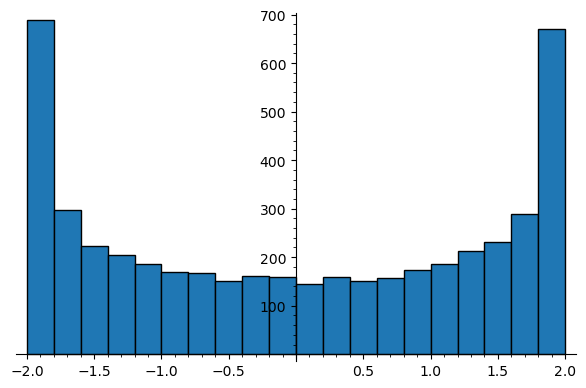
\includegraphics[height=2in]{E1.png}
	\end{center}
\end{example}
\begin{example} \label{ex:sato-tate-distribution-e2}
	Here is a histogram of the values of $a_p(E_2)$ for $p<10^5$.
	\begin{center}
		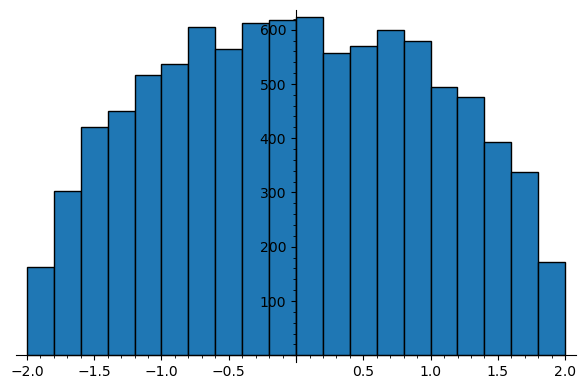
\includegraphics[height=2in]{E2.png}
	\end{center}
\end{example}
These are remarkable histograms! We encourage the reader to investigate other elliptic curves.
\begin{remark}
	It turns out that ``most of the time'' we will get a semicircle distribution as in \Cref{ex:sato-tate-distribution-e2}.
\end{remark}
A primary goal of the talk is to explain the source of these strange curves.

\subsection{The Weil Conjectures} \label{subsec:weil}
This subsection is included for motivational purposes only and can therefore be skipped without loss of too much continuity.

It will turn out that the values of $a_p(E)$ are controlled by a Galois representation attached to $E$. The most concrete way to construct this Galois representation is to use the Tate module, which we will do shortly. However, for motivation, we will state the Weil conjectures and explain how they solve our problem.
\begin{theorem}[Weil conjectures] \label{thm:weil-conj}
	Fix a smooth projective variety $X$ over a finite field $\FF_q$ of dimension $n$. Then the formal power series
	\[\zeta_X(T)\coloneqq\exp\Bigg(\sum_{r=1}^\infty\#X\left(\FF_{q^r}\right)\frac{T^r}r\Bigg)\]
	admits the following desirable properties.
	\begin{listalph}
		\item Rationality: one can write
		\[\zeta_X(T)=\frac{P_1(T)\cdots P_{2n-1}(T)}{P_2(T)\cdots P_{2n}(T)}\]
		for polynomials $P_\bullet(T)\in 1+T\ZZ[T]$.
		\item Riemann hypothesis: the roots of the polynomial $P_\bullet(T)$ are complex numbers with roots of magnitude $q^{-\bullet/2}$.
		\item Betti numbers: suppose $X$ is the reduction of a smooth projective variety $\mc X$ defined over a number ring $\OO_K$. Then $\deg P_\bullet=\dim_\CC H^\bullet(\mc X(\CC),\CC)$.
	\end{listalph}
\end{theorem}
We will not bother to explain why $\zeta_X(T)$ is the correct $\zeta$-function to look at (roughly speaking, one is supposed to plug in $T\coloneqq q^{-s}$).

The mention of Betti numbers is rather compelling because it suggests that there ought to be a way to write down a cohomology theory for smooth projective varieties $X$. Without going into too much detail, let's explain how this is done. It is possible to define a satisfactory cohomology theory called ``$\ell$-adic cohomology'' which takes as input an auxiliary prime $\ell$ which is nonzer in $\FF_q$ and then is able to (functorialy) produce cohomology groups $H^\bullet(X,\QQ_\ell)$ which are $\QQ_\ell$-vector spaces. For example, in the situation of \Cref{thm:weil-conj}(c), we find that
\[\dim_{\QQ_\ell} H^\bullet(X,\QQ_{\ell})=\dim_\CC H^\bullet(\mc X(\CC),\CC).\]
Now, for \Cref{thm:weil-conj}, the main point is to be able to compute $\#X(\FF_q)$. Well, the main idea is that $X(\FF_q)$ consists of the elements of $X(\overline{\FF_q})$ which are fixed by the Frobenius morphism $\op{Frob}_q\colon\overline{\FF_q}\to\overline{\FF_q}$. Thus, one can use the Lefschetz trace formula on our cohomology theory $H^\bullet(X,\QQ_\ell)$ to find
\[\#X(\FF_q)=\sum_{i=0}^{2d}(-1)^i\tr\left({\op{Frob}_q}\vert H^i(X,\QQ_\ell)\right).\]
Properties of the cohomology theory are then enough to prove the Weil conjectures purely formally.

For example, in the case of a curve $C$, we find that
\[\#C(\FF_q)=q+1-\tr\left({\op{Frob}_q}\vert H^1(C,\QQ_\ell)\right),\]
so we become interested in the Galois action on some $\ell$-adic vector space $H^1(C,\QQ_\ell)$. In the following section, we will provide a direct construction for (the dual of) $H^1(E,\QQ_\ell)$ for an elliptic curve $E$.
\begin{exe}
	Use the above discussion to prove \Cref{thm:hasse-weil}.
\end{exe}

\subsection{The Tate Module for Elliptic Curves} \label{subsec:tate-module-ecs}
We now go on the hunt for a Galois representation attached to $E$, where $E$ continues to be an elliptic curve defined over $\QQ$ (with a suitable integral model). It turns out that there basically one way to do this, though the recipe is somewhat roundabout. Something special about $E$ is that it comes with a group law, which means that $E(R)$ is a group (in a functorial way) for all $\QQ$-algebras $R$. For example, \Cref{ex:ec-as-c-mod-lattice} realized $E(\CC)$ as $\CC/\Lambda$ for some lattice $\Lambda$, and the group law on $\CC/\Lambda$ is the expected one.

As such, we note that $E(\overline\QQ)$ is a group with an action by $\op{Gal}(\overline\QQ/\QQ)$. One can see this purely by the ambient functoriality; alternatively, one can directly construct this action by noting that $E(\overline\QQ)\subseteq\PP^2_\QQ(\overline\QQ)$, and of course $\PP^2_\QQ(\overline\QQ)$ has a Galois action by acting on the coordinates:
\[\sigma([X:Y:Z])\coloneqq[\sigma(X):\sigma(Y):\sigma(Z)]\]
for all $\sigma\in\op{Gal}(\overline\QQ/\QQ)$ and $[X:Y:Z]\in\PP^2_\QQ(\overline\QQ)$.

However, in order to do linear algebra, we want our Galois representation to be valued in a vector space. Thus, the Galois action on $E(\overline\QQ)$ will not quite work. As such, we will want the following fact about the group law; throughout, $G[n]$ denotes the $n$-torsion of a group $G$.
\begin{proposition} \label{prop:torsion-of-ec}
	Fix an elliptic curve $E$ defined over an algebraically closed field $\overline K$. For any $n$ which is nonzero in $K$, there is a non-canonical isomorphism
	\[E(\ov K)[n]\cong(\ZZ/n\ZZ)^2.\]
\end{proposition}
\begin{example}
	For $E=\CC/\Lambda$, it is not hard to show that $E[n]$ is a group isomorphic to $(\ZZ/n\ZZ)^2$. In particular, as abstract groups, one finds that $\CC\cong\Lambda\otimes_\ZZ\RR$, so
	\[E\cong(\RR/\ZZ)^2,\]
	whose $n$-torsion has the desired property.
\end{example}
This is slightly better: for any prime $\ell$, we see that $E(\overline\QQ)[\ell]$ is a $2$-dimensional $\FF_\ell$-vector space, and more generally, $E(\overline\QQ)[\ell^\bullet)$ is a free module over $(\ZZ/\ell^\bullet\ZZ)$ of rank $2$. In order to not have to deal with torsion, we take an inverse limit.
\begin{definition}[Tate module]
	Fix an elliptic curve $E$ defined over an algebraically closed field $\overline K$. For any prime $\ell$ nonzero in $K$, we define the \textit{Tate module} as the inverse limit
	\[T_\ell E\coloneqq\limit E\left[\ell^\bullet\right],\]
	where the transition maps $E\left[\ell^{\bullet+1}\right]\onto E\left[\ell^\bullet\right]$ are given by multiplication by $\ell$. We also define $V_\ell E\coloneqq T_\ell E\otimes_\ZZ\QQ$.
\end{definition}
\begin{remark}
	We see that $T_\ell E$ is non-canonically isomorphic to $\ZZ_\ell^2$, so $V_\ell E$ is non-canonically isomorphic to $\QQ_\ell^2$.
\end{remark}
\begin{remark}
	Intuitively, one should think about $T_\ell E$ as a complex-analytic version of $H_1(E,\ZZ)$. For example, $(V_\ell E)^\lor$ should be analogous to $H^1(E,\QQ)$.
\end{remark}
The Galois action of $\op{Gal}(\overline\QQ/\QQ)$ on each $E(\overline\QQ)\left[\ell^\bullet\right]$ will now assemble into a Galois action on $T_\ell E$ and thus $V_\ell E$, so we have produced a homomorphism
\[\rho_\ell\colon\op{Gal}(\overline\QQ/\QQ)\to\op{GL}(V_\ell E).\]
It is rather difficult to compute this Galois representation directly, but it knows quite a bit about the arithmetic of $E$.
\begin{proposition} \label{prop:char-polys-on-h1}
	Fix an elliptic curve $E$ defined over a field $K$, and let $\ell$ be a prime nonzero in $K$. For any endomorphism $\varphi\colon E\to E$, let $P_\ell(T)$ be the monic characteristic polynomial of $\varphi$ acting on $V_\ell E$. For each $n\in\ZZ$, the number $P_\ell(n)$ is independent of $\ell$ and equals the degree of the map $\varphi-[n]$, where $[n]\colon E\to E$ is multiplication by $n$.
\end{proposition}
\begin{example}
	Let's compare this with what we expect to happen for $H_1(E,\ZZ)$ when $E=\CC/\Lambda$. Then $H_1(E,\ZZ)=\Lambda$, so the characteristic polynomial $P_\varphi$ of some endomorphism $\varphi\colon E\to E$ will satisfy
	\begin{align*}
		\left|P_\varphi(n)\right| &= \left|\det\left(\varphi-[n]\vert H_1(E,\ZZ)\right)\right| \\
		&= \left|\det\left(\varphi-[n]\vert \Lambda\right)\right| \\
		&= \#\left(\frac{\Lambda}{(\varphi-[n])\Lambda}\right) \\
		&= \#\left(\frac{(\varphi-[n])^{-1}\Lambda}\Lambda\right) \\
		&= \#\ker(\varphi-[n]) \\
		&= \deg(\varphi-[n]).
	\end{align*}
\end{example}
Here are two examples.
\begin{corollary} \label{cor:char-poly-frob}
	Fix an elliptic curve $E$ defined over $\QQ$ with a good enough integral model, and let $\ell$ be a prime. For a prime $p\ne\ell$, let $P_\ell(T)$ be the characteristic polynomial of $\rho_\ell({\op{Frob}_p})$, for any choice of $\op{Frob}_p$ in the conjugacy class of $\op{Gal}(\overline\QQ/\QQ)$. Then
	\[P_\ell(0)=p\qquad\text{and}\qquad P_\ell(1)=\#E(\FF_p).\]
\end{corollary}
\begin{proof}
	Let $F\colon A(\overline{\FF_p})\to A(\overline{\FF_p})$ be given by the action of $\op{Frob}_p$. \Cref{prop:char-polys-on-h1} tells us that $P_\ell(0)$ equals the degree of $F$, which is $p$ because it corresponds to the degree of some field extension which looks like $K(t^p)\subseteq K(t)$. Similarly, we see $P_\ell(1)$ equals the degree of the map $F-\id_E$, which is the number of points fixed by $F$, which is the size of $E(\FF_p)$.
\end{proof}
In particular, in the situation of the corollary, we are able to compute that
\[P_\ell(T)=T^2-aT+p,\]
where $a=(p+1)-\#E(\FF_p)$. Factoring $P_\ell(T)=(T-\alpha_{1})(T-\alpha_2)$, we find that
\[\frac1{\sqrt p}\tr\rho_\ell({\op{Frob}_p})=\frac{\alpha_1+\alpha_2}{\sqrt p}=\frac{(p+1)-\#E(\FF_p)}{\sqrt p}=a_p(E).\]
Thus, our Galois representation is good enough to understand our desired numbers $a_p(E)$!

\subsection{Defining the Sato--Tate Group: Elliptic Curves}
We continue with our elliptic curve $E$ defined $\QQ$, and we fix our auxiliary prime $\ell$. The moral of the story is that we can measure the distribution of $a_p(E)$s via the distribution of $\rho_\ell(\mathrm{Frob}_p)$; we then recover the distribution of the $a_p(E)$s by taking the trace.

Once again, we may guess that the $\rho_\ell({\mathrm{Frob}_p})$s must equidistribute in $\op{GL}(V_\ell E)\cong\op{GL}_2(\QQ_\ell)$. However, this cannot be the case because
\[\det\rho_\ell({\mathrm{Frob}_p})=p\]
by \Cref{cor:char-poly-frob}. Thus, we would like to rescale $\rho_\ell({\op{Frob}_p})$ to account for this determinant condition. Namely, we would like to replace $\rho_\ell({\mathrm{Frob}_p})$ with $\frac1{\sqrt p}\rho_\ell({\mathrm{Frob}_p})$, but there is no reasonable way to do this because $\QQ_\ell$ may not have the element $1/\sqrt p$ for all the primes $p$ we want to look at. And even when it does, there are two reasonable square roots to look at, so it is not obvious which one to choose: a different choice will lead to a different trace!

To fix this problem, we cheat: we choose any embedding $\iota\colon\QQ_\ell\into\CC$, which exists because these two fields have the same cardinality, and $\CC$ is algebraically closed. Then we may hope that the elements
\[\frac1{\sqrt p}\iota(\rho_\ell({\mathrm{Frob}_p}))\in\op{SL}_2(\CC)\]
will equidistribute as $p$ varies. However, this still cannot be the case because $\rho_\ell$ is a continuous map with compact source $\op{Gal}(\overline\QQ/\QQ)$, so these elements should actually live in some compact group. As such, we fix the compact subgroup ${\op{SU}_2}\subseteq\op{SL}_2(\CC)$, and we hope that the elements
\[\frac1{\sqrt p}\iota(\rho_\ell({\mathrm{Frob}_p}))\in{\op{SU}_2}\]
will equidistribute. Technically, this does not really make sense because $\op{Frob}_p$ was only defined up to conjugacy, so the element $\frac1{\sqrt p}\iota(\rho_\ell({\mathrm{Frob}_p}))$ will also only be defined up to conjugacy, so we are really hoping that the elements
\[\left[\frac1{\sqrt p}\iota(\rho_\ell({\mathrm{Frob}_p}))\right]\in\op{Conj}({\op{SU}_2})\]
will equidistribute.

This is generally true.
\begin{example}
	For the curve $E_2\colon y^2=x^3+x+1$, it will turn out that the conjugacy classes
	\[\left[\frac1{\sqrt p}\iota(\rho_\ell({\mathrm{Frob}_p}))\right]\in\op{Conj}({\op{SU}_2})\]
	do equidistribute in $n\op{Conj}({\op{SU}_2})$. This is the ``generic'' case for our elliptic curves, and one can show that this equidistribution gives rise to the semicircle distribution seen in \Cref{ex:sato-tate-distribution-e2} upon applying the trace.
\end{example}
In fact, one has the following.
\begin{theorem}[Sato--Tate, non-CM elliptic curve]
	Fix an elliptic curve $E$ defined over $\QQ$, and let $\ell$ be an auxiliary prime, and let $\iota\colon\QQ_\ell\to\CC$ be some embedding. Let $\rho_\ell$ be the Galois representation given by $V_\ell E$. Assume $\op{End}(E_{\overline\QQ})=\ZZ$. Then the elements
	\[\left\{\frac1{\sqrt p}\iota(\rho_\ell({\op{Frob}_p}))\right\}_{p\text{ prime}}\]
	equidistribute among the conjugacy classes of $\op{SU}_2$.
\end{theorem}
\begin{remark}
	Perhaps we ought to explain what it means to equistribute in $\op{Conj}({\op{SU}_2})$. Well, $\op{SU}_2$ is a compact topological group, so it has a Haar measure, and there is a procedure to push this measure forward along the canonical projection.
\end{remark}
The difference between \Cref{ex:sato-tate-distribution-e1,ex:sato-tate-distribution-e2} imply that we cannot expect the above discussion to be true for all elliptic curves.

To explain what is going on, note that $E_1\colon y^2=x^3+1$ has a bizarre extra endomorphism $\varphi\colon E_1\to E_1$ given by
\[\varphi(x,y)\coloneqq(\zeta_3x,y).\]
This endomorphism is defined over $\QQ(\zeta_3)$, which means that whenever ${\op{Frob}_p}\in\op{Gal}(\overline\QQ/\QQ(\zeta_3))$, we will have
\[\rho_\ell(\varphi)\circ\rho_\ell({\op{Frob}_p})=\rho_\ell({\op{Frob}_p})\circ\rho_\ell(\varphi).\]
Thus, we do not expect our elements to equidistribute in $\overline{\op{SU}_2}$: there should be an extra condition to account for commuting with endomorphisms (possibly defined over an extension of $\QQ$).

The general way to account for this is to simply ignore it. We have the following definition.
\begin{definition}[$\ell$-adic monodromy group]
	Fix an elliptic curve $E$ defined over $\QQ$, and let $\ell$ be an auxiliary prime. Let $G_\ell$ be the image of $\rho_\ell$, and let $G_\ell^{\mathrm{Zar}}$ be the smallest algebraic subgroup of $\op{GL}_{2}(\QQ_\ell)$ which is defined over $\QQ_\ell$ containining $G_\ell$. We call $G_\ell^{\mathrm{Zar}}$ the \textit{$\ell$-adic monodromy group}.
\end{definition}
We can now define the Sato--Tate group $\op{ST}(E)$ by retelling the above story.
\begin{definition}[Sato--Tate group]
	Fix an elliptic curve $E$ defined over $\QQ$, and let $\ell$ be an auxiliary prime. Let $G_\ell^{\mathrm{Zar},1}$ be the subgroup of $G_\ell^{\mathrm{Zar}}$ cut out by the condition that the determinant equals $1$. Then the \textit{Sato--Tate group} is a maximal compact subgroup of $G_\ell^{\mathrm{Zar},1}(\CC)$, where we take $\CC$-points via some embedding $\QQ_\ell\subseteq\CC$.
\end{definition}
And here is the theorem, due to Richard Taylor and many other people.
\begin{theorem}[Sato--Tate, elliptic curve] \label{thm:st-ec}
	Fix an elliptic curve $E$ defined over $\QQ$, and let $\ell$ be an auxiliary prime, and let $\iota\colon\QQ_\ell\to\CC$ be some embedding. Then the elements
	\[\left\{\frac1{\sqrt p}\iota(\rho_\ell({\op{Frob}_p}))\right\}_{p\text{ prime}}\]
	equidistribute among the conjugacy classes of $\op{ST}(E)$.
\end{theorem}
\begin{remark} \label{rem:why-in-st}
	It is not totally clear why $\frac1{\sqrt p}\iota(\rho_\ell({\op{Frob}_p}))$ would even be conjugate to any element in $\op{ST}(E)$. Roughly speaking, we are combining two properties.
	\begin{enumerate}
		\item It turns out that $\rho_\ell({\op{Frob}_p})$ is diagonalizable over an algebraic closure. Thus, our element (with eigenvalues of absolute value $1$) it certainly contained in some compact subgroup.
		\item Over $\CC$, it turns out that any compact subgroup is conjugate to a subgroup of a given maximal compact subgroup. Thus, we can conjugate our element into $\op{ST}(E)$.
	\end{enumerate}
\end{remark}
\begin{example}
	For $E_1$, one shows that $\op{ST}(E_1)$ is a normalizer of $\op U_1$ diagonally embedded in $\op{SU}_2$. Roughly speaking, the point is that the field $\QQ(\zeta_3)$ has an action on $V_\ell E_1$ which commutes with the Galois action restricted to $\op{Gal}(\overline\QQ/\QQ(\zeta_3))$, which causes the Galois action to diagonalize.
\end{example}

\subsection{The Sato--Tate Conjecture: Abelian Varieties}
In order to wrap up our story, we note that our discussion of Sato--Tate groups for elliptic curves generalizes to abelian varieties without too much effort.
\begin{definition}[abelian variety]
	Fix a field $K$. Then an \textit{abelian variety} $A$ over $K$ is a smooth projective geometrically integral group variety over $K$.
\end{definition}
Here, being a group variety means that $A(R)$ is a group (in a functorial way) for all $K$-alegbras $R$, as we had for elliptic curves.
\begin{example}
	Any product of elliptic curves continues to be an abelian variety. The category of abelian varieties is in fact abelian, so we can also take kernels and cokernels.
\end{example}
\begin{example}
	Fix a nonnegative integer $g$. Then for some lattices $\Lambda\subseteq\CC^g$, it turns out that the quotient $\CC^g/\Lambda$ is a projective variety over $\CC$, so this is an abelian variety over $\CC$ with the obvious group law.
\end{example}
Let's make explicit how the discussion of the previous two subsections generalizes to abelian varieties. Here is the generalization of \Cref{prop:torsion-of-ec}.
\begin{proposition}
	Fix an abelian vareity $A$ over a field $K$ of dimension $g$. For any $n$ which is nonzero in $K$, there is a non-canonical isomorphism
	\[A(\overline K)[n]\cong(\ZZ/n\ZZ)^{2g}.\]
\end{proposition}
This allows us to define the Tate module as before.
\begin{definition}[Tate module]
	Fix an abelian variety $A$ defined over a field $K$. For any prime $\ell$ nonzero in $K$, we define the \textit{Tate module} as the inverse limit
	\[T_\ell A\coloneqq\limit A\left[\ell^\bullet\right].\]
	We also define $V_\ell A\coloneqq T_\ell A\otimes_\ZZ\QQ$. As before, we find that $T_\ell A$ is a free module over $\ZZ_\ell$ of rank $2g$.
\end{definition}
Thus, as before, we get an $\ell$-adic Galois representation
\[\rho_\ell\colon\op{Gal}(\overline\QQ/\QQ)\to\op{GL}(V_\ell A).\]
We can also generalize some of our discussion about the characteristic polynomial. Here is the generalization of \Cref{cor:char-poly-frob}.
\begin{proposition}
	Fix an abelian variety $A$ defined over $\QQ$ with a good enough integral model, and let $\ell$ be a prime. For a prime $p\ne\ell$, let $P_\ell(T)$ be the characteristic polynomial of $\rho_\ell({\op{Frob}_p})$, for any choice of $\op{Frob}_p$ in the conjugacy class of $\op{Gal}(\overline\QQ/\QQ)$. Then $P_\ell(T)$ is a polynomial independent of $\ell$, and
	\[P_\ell(0)=p^g\qquad\text{and}\qquad P_\ell(1)=\#A(\FF_p).\]
\end{proposition}
Thus, our discussion defining $\op{ST}(E)$ can be generalized to build $\op{ST}(A)$, as follows.
\begin{enumerate}
	\item Let $G_\ell(A)$ be the image of $\rho_\ell$ in $\op{GL}(V_\ell A)$, and let $G_\ell^{\mathrm{Zar}}(A)$ be the smallest algebraic subgroup defined over $\QQ_\ell$ containing $G_\ell$.
	\item By choosing a Weil pairing on $T_\ell A$ (which we will not define), it turns out that there is a non-degenerate symplectic form on $V_\ell A$, and $\rho_\ell({\op{Frob}_p})$ acts with multiplier $p$ with respect to this form. Thus, we let $G_\ell^{\mathrm{Zar},1}(A)$ be the subgroup of $G_\ell^{\mathrm{Zar}}(A)$ cut out by preserving the corresponding symplectic form.
	\item Choose some embedding $\iota\colon\QQ_\ell\to\CC$. We now let $\op{ST}(A)$ be a maximal compact subgroup of the complex algebraic group $\iota\left(G_\ell^{\mathrm{Zar},1}(A)\right)$.
\end{enumerate}
And here is the conjecture.
\begin{conj}[Sato--Tate] \label{conj:st}
	Fix an abelian variety $A$ defined over $\QQ$, and let $\ell$ be an auxiliary prime, and let $\iota\colon\QQ_\ell\to\CC$ be some embedding. Let $\rho_\ell$ be the Galois representation given by $V_\ell A$. Then the elements
	\[\left\{\frac1{\sqrt p}\iota(\rho_\ell({\op{Frob}_p}))\right\}_{p\text{ prime}}\]
	equidistribute among the conjugacy classes of $\op{ST}(A)$.
\end{conj}
\Cref{rem:why-in-st} once again explains why our elements have a conjugacy class in $\op{ST}(A)$. Also, note that this is a conjecture unlike \Cref{thm:st-ec}!

\subsection{Jacobian Varieties}
In order to provide some examples of abelian varieties, we introduce Jacobian varieties into our story. In order to avoid doing any difficult algebraic geometry or complex geometry, we will define these by universal property.
\begin{proposition} \label{prop:jac-up}
	Fix a curve $C$ defined over a field $K$ equipped with a point $x\in C(K)$. Then there exists an abelian variety $\op{Jac}(C)$ equipped with a map $C\into\op{Jac}(C)$ sending $x\mapsto0$ and satisfying the following the corresponding universal property: for any abelian variety $A$ and morphism $\varphi\colon C\to A$ sending $\varphi(x)=0$, there exists a unique map $\widetilde\varphi\colon\op{Jac}(C)\to A$ making the following diagram commute.
	% https://q.uiver.app/#q=WzAsMyxbMCwwLCJDIl0sWzEsMCwiXFxvcHtKYWN9KEMpIl0sWzEsMSwiQSJdLFswLDIsIlxcdmFycGhpIiwyXSxbMSwyLCJcXHdpZGV0aWxkZVxcdmFycGhpIiwwLHsic3R5bGUiOnsiYm9keSI6eyJuYW1lIjoiZGFzaGVkIn19fV0sWzAsMSwiIiwwLHsic3R5bGUiOnsidGFpbCI6eyJuYW1lIjoiaG9vayIsInNpZGUiOiJ0b3AifX19XV0=&macro_url=https%3A%2F%2Fraw.githubusercontent.com%2FdFoiler%2Fnotes%2Fmaster%2Fnir.tex
	\[\begin{tikzcd}
		C & {\op{Jac}(C)} \\
		& A
		\arrow[hook, from=1-1, to=1-2]
		\arrow["\varphi"', from=1-1, to=2-2]
		\arrow["{\widetilde\varphi}", dashed, from=1-2, to=2-2]
	\end{tikzcd}\]
\end{proposition}
\begin{definition}[Jacobian]
	Fix a curve $C$ defined over a field $K$ equipped with a point $x\in C(K)$. Then the abelian variety $\op{Jac}(C)$ produced by \Cref{prop:jac-up} is called the \textit{Jacobian} of $C$.
\end{definition}
\begin{example}
	For an elliptic curve $E$, we see that $\op{Jac}(E)=E$ because $E$ is already an abelian variety.
\end{example}
\begin{example}
	Let's give the construction for $\op{Jac}(C)$ when our curve $C$ is defined over $\CC$. One can embed the first homology $H_1(C,\ZZ)$ into the complex vector space $H^0(C,\Omega^1_C)^\lor$ by taking $[\gamma]\in H_1(C,\ZZ)$ to the functional
	\[\omega\mapsto\int_\gamma\omega.\]
	Then $\op{Jac}(C)=H^0(C,\Omega^1_C)^\lor/H_1(C,\ZZ)$.
\end{example}
\begin{remark}
	It is not obvious from the definition, but it turns out that the dimension of $\op{Jac}(C)$ equals the genus of the curve $C$.
\end{remark}
\begin{remark}
	Motivated by \cref{subsec:weil}, the importance of the Jacobian arises from the fact that the map $C\to\op{Jac}(C)$ induces an isomorphism
	\[H^1(\op{Jac}(C),\QQ_\ell)\to H^1(C,\QQ_\ell)\]
	on first cohomology. In particular, we can hope to read off properties of the curve (related to its cohomology) from the Jacobian. The analogous statement for $\CC$ is simply that $H_1(C,\ZZ)\to H_1(\op{Jac}(C),\ZZ)$ is an isomorphism, which is clear from our construction.
\end{remark}
The following result follows from the discussion in \cref{subsec:weil} and the above remark.
\begin{proposition}
	Fix a curve $C$ defined over $\QQ$ with a good enough integral model, and set $A\coloneqq\op{Jac}(C)$. For any prime $p$ and an auxiliary prime $\ell\ne p$, we have
	\[\#C(\FF_p)-(p+1)=\tr\left(\rho_\ell({\op{Frob}_p})\vert V_\ell A\right)\]
\end{proposition}
Thus, we expect computable (but perhaps complicated) equidistribution results for general curves to follow from \Cref{conj:st}. Here is one such histogram.
\begin{example}
	Consider the genus-$2$ curve $C\colon y^2=x^5+x+1$. Here is a histogram for the values of $a_p(C)\coloneqq(\#C(\FF_p)-(p+1))/\sqrt p$ for $p<10^5$.
	\begin{center}
		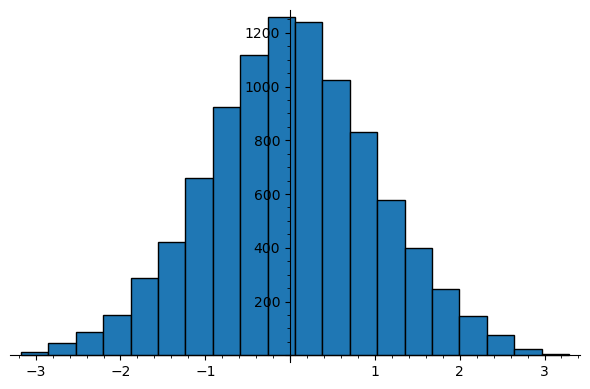
\includegraphics[height=2in]{hyper.png}
	\end{center}
\end{example}

\section{CM Theory}
In our second talk, we will use the theory of complex multiplication to discuss how to compute $\op{ST}(A)$ for certain abelian varieties $A$.

\subsection{Algebraic Tori}
In this subsection, we recall some facts about algebraic tori.
\begin{definition}[algebraic torus]
	Fix a field $k$ with separable closure $k^{\mathrm{sep}}$. Then an \textit{algebraic torus} is a connected algebraic group scheme $T$ over $k$ such that $T_{k^{\mathrm{sep}}}\cong\mathbb G_{m,k^{\mathrm{sep}}}^r$ for some $r\ge0$; we say that $r$ is the \textit{rank} of $T$, sometimes denoted $\op{rank}(T)$.
\end{definition}
\begin{remark}
	Importantly, the isomorphism $T\cong\mathbb G_m^r$ need note be defined over $k$.
\end{remark}
\begin{example}[Deligne torus]
	Consider the group $\mathbb S\coloneqq\op{Res}_{\CC/\RR}\mathbb G_{m,\CC}$, which is an algebraic group defined over $\RR$ such that $\mathbb S(\RR)\cong\CC^\times$. Explicitly, we can write
	\[\mathbb S(R)=\left\{\begin{bmatrix}
		a & -b \\
		b & a
	\end{bmatrix}\in M_2(R):a^2+b^2\in R^\times\right\},\]
	for any $\RR$-algebra $R$. Then one can check that $\mathbb S(\CC)\cong\CC^\times\times\CC^\times$, which actually assembles into an isomorphism of algebraic groups
	\[\mathbb S_\CC\cong\mathbb G_{m,\CC}\times\mathbb G_{m,\CC}.\]
\end{example}
\begin{example}
	More generally, for any finite separable field extension $E/F$, one can define a torus $T_{E/F}\coloneqq\op{Res}_{E/F}\mathbb G_{m,E}$, and then one finds that $T_{E/F}\otimes_FE\cong\mathbb G_{m,E}^{[E:F]}$. Roughly speaking, one upgrades the isomorphism
	\[E\otimes_FF^{\mathrm{sep}}\cong E^{\op{Hom}(E,F^{\mathrm{sep}})}\]
	to an isomorphism of algebraic groups. (This isomorphism uses the primitive element theorem, which is why $E/F$ is required to be separable.)
\end{example}
Given a torus $T$, we define the groups
\[X^*(T)\coloneqq\op{Hom}(T_{k^{\mathrm{sep}}},\mathbb G_m)\qquad\text{and}\qquad X_*(T)\coloneqq\op{Hom}(\mathbb G_m,T_{k^{\mathrm{sep}}}),\]
which are the character and cocharacter groups, respectively. Because $T_{k^{\mathrm{sep}}}\cong\mathbb G_m^r$ for some $r\ge0$, we see that these are both free abelian groups with rank $r$. However, there is also an important Galois action by $\op{Gal}(k^{\mathrm{sep}}/k)$ on both of these groups via its action on $T_{k^{\mathrm{sep}}}$.
\begin{example} \label{ex:char-s}
	We can define two characters $\mathbb S_\CC\to\mathbb G_m$ given on points
	\[\CC^\times=\mathbb S(\RR)\subseteq\mathbb S(\CC)\to\mathbb G_m(\CC)\]
	by $z\mapsto z$ and $z\mapsto\overline z$. One can check that these two characters span $X^*(\mathbb S)$, and the nontrivial Galois action of complex conjugation in $\op{Gal}(\CC/\RR)$ simply swaps these two characters.
\end{example}
\begin{example}
	Similarly, fix a number field $E$, and consider the torus $T_E\coloneqq\op{Res}_{E/\QQ}\mathbb G_m$. For each $\varphi\in\op{Hom}(E,\overline\QQ)$, define we define a character of $T_E$ given by projection onto the $\varphi$ coordinate in the isomorphism
	\[E\otimes_\QQ\overline\QQ\cong\overline\QQ^{\op{Hom}(E,\overline\QQ)}\]
	of algebras with Galois action. In this way, we find that $X^*(T_E)=\ZZ[\op{Hom}(E,\CC)]$, which is an isomorphism of Galois modules. Note that one can then construct a dual basis $\varphi^\lor$ of $X_*(T_E)$.
\end{example}
The importance of the character group is the following result.
\begin{theorem}
	Fix a field $k$. The contravariant functor $X_*$ defines an anti-equivalence of categories between the category of algebraic tori (over $k$) and free abelian groups of finite rank which are $\op{Gal}(k^{\mathrm{sep}}/k)$-modules.
\end{theorem}
\begin{remark}
	There is an analogous result for the covariant functor $X_*$.
\end{remark}
Roughly speaking, the idea is that (over $k^{\mathrm{sep}}$) one can understand tori perfectly by their maps to $\mathbb G_m$ because one really only cares about rank. To descend to $k$, one then needs to keep track of the Galois action.

\subsection{A Little Hodge Theory}
Before doing anything too intense, we will discuss some Hodge theory.
\begin{definition}[Hodge structure]
	Fix an integer $n$. A \textit{Hodge structure} over $\QQ$ is a $\QQ$-vector space equipped with a decomposition
	\[V_\CC=\bigoplus_{(p,q)\in\ZZ^2}V^{p,q}\]
	such that $V^{p,q}=\overline{V^{q,p}}$. If $V^{p,q}\ne0$ only when $p+q=n$, then we say that $V$ is \textit{pure of weight $n$}.
\end{definition}
\begin{remark}
	There is also a notion of an integral Hodge structure, where we make $\ZZ$ into a free $\ZZ$-module instead of a $\QQ$-vector space.
\end{remark}
Here is the key example.
\begin{example}
	Fix a smooth proper complex variety $X$ over $\CC$. Then the cohomology group $H^n(X(\CC),\QQ)$ admits a Hodge decomposition as
	\[H^n(X(\CC),\QQ)\otimes_\QQ\CC=\bigoplus_{p+q=n}H^{p,q},\]
	where $H^{q,p}=H^q(X(\CC),\Omega_{X/\CC}^p)$.
\end{example}
\begin{example}
	We are interested in abelian varieties $A$. Then all cohomology is generated by $H^1$, so it will be enough to understand the Hodge structure there. Thus, for an abelian variety $A$, we note that there is a Hodge structure on $H_1(A,\QQ)$ of weight $-1$. (The weight negates because we are now looking at homology.)
\end{example}
Intuitively, Hodge theory is the extra structure on cohomology provided by complex geometry, in the same way that Galois theory is the extra structure on cohomology provided by the \'etale site.

The reason we are bringing up this Hodge theory is that we will be able to compute the complex analytic version of the $\ell$-adic monodromy group $G_\ell(A)$. For this, we will need a representation-theoretic interpretation of a Hodge structure.
\begin{lemma}
	Fix a vector space $V$ defined over $\QQ$. The data of a Hodge structure on $V$ is equivalent to the data of a representation $\rho\colon\mathbb S\to\op{GL}(V_\RR)$.
\end{lemma}
\begin{proof}
	The point is to describe what representations look like. Over $\mathbb S_\CC$, we see that the representation $\rho$ will diagonalize as a representation $\mathbb G_{m,\CC}^2\to\op{GL}(V_\CC)$. Thus, we can decompose
	\[V_\CC=\bigoplus_{\chi\in X^*(\mathbb S)}V_\chi,\]
	where $V_\chi$ is the $\chi$-eigenspace. Now, each character $\chi$ can be written as $z\mapsto z^{-p}\overline z^{-q}$ for some $(p,q)\in\ZZ^2$ where $z,\overline z\in X^*(\mathbb S)$ are the characters of \Cref{ex:char-s}, so we let $V^{p,q}$ be the eigenspace for this character. As such, we see that the nontrivial Galois action of complex conjugation in $\op{Gal}(\CC/\RR)$ will swap $V^{p,q}$ and $V^{q,p}$, so $V^{p,q}=\overline{V^{q,p}}$. Thus, we see that we have produced a Hodge structure on $V$; one can then reverse this construction to produce a representation of $\mathbb S$ from any given Hodge structure.
\end{proof}
Now that we have a representation, we can take monodromy.
\begin{definition}[Mumford--Tate group]
	Fix a Hodge structure over $\QQ$ on a vector space $V$. Then the \textit{Mumford--Tate group} $\op{MT}(V)$ is the smallest connected algebraic group defined over $\QQ$ containing the image of $h\colon\mathbb S\to\op{GL}(V_\RR)$. For brevity, given an abelian variety $A$ defined over $\CC$, we may write $\op{MT}(A)$ for the Mumford--Tate group of the Hodge structure on $H_1(A,\QQ)$.
\end{definition}
\begin{remark}
	There is also an important Tannakian definition of $\op{MT}(V)$. In short, the category of Hodge structures over $\QQ$ is neutral Tannakian, so for any Hodge structure $V$, we can look at the Tannakian subcategory generated by $V$. Then $\op{MT}(V)$ is the algebraic group given by this category.
\end{remark}
\begin{remark}
	Because an algebraic group can be described by the vectors it fixes, the above definition can be restated as follows: $\op{MT}(V)$ is the subgroup such that a rational subquotient $W$ of some sum of $V$s and $V^\lor$s is a Hodge substructure if and only if $W$. For example, this allows one to see that $\op{MT}(V)\subseteq\op{GL}(V)$ must contain the scalar matrices.
\end{remark}
\begin{remark}
	For an abelian variety $A$, it turns out that $\op{MT}(A)$ is always reductive. Roughly speaking, this follows from the fact that $A$ has a polarization, so $H_1(A,\QQ)$ is a polarizable Hodge structure.
\end{remark}
It is at this point that one would expect me to write down some basic examples of Mumford--Tate groups, but this turns out to be a fairly difficult task. For example, because we are looking at the image of some torus $\mathbb S$, one may expect that $\op{MT}(V)$ is frequently a torus. In our application (in the CM theory), this will turn out to be the case, but this is exceptional: most of the time we expect $\op{MT}(V)$ to be large (largely because the algebraic group needs to descend all the way $\QQ$), though this is not always easy to prove.

Nonetheless, let us give a couple remarks bounding $\op{MT}(A)$.
\begin{remark} \label{rem:endo-mt-bound}
	For brevity, set $V\coloneqq H_1(A,\QQ)$ and $D\coloneqq\op{End}(A)\otimes_\ZZ\QQ$, which one can show is a product of division algebras over $\QQ$. It turns out that endomorphisms of $A$ then correspond to endomorphisms of $V$ preserving the Hodge structure. However, an endomorphism of $V$ preserving the Hodge structure turns out to be the same data of an element of $V\otimes V^\lor$ which is fixed by the image of $h$, which of course is equivalent to being fixed by $\op{MT}(A)$. Thus, we see that
	\[\op{End}(V)^{\op{MT}(A)}=\op{End}(A).\]
	Thus, we see that we have a lower bound that $\op{MT}(A)$ will be contained with the subgroup of $\op{GL}(V)$ commuting with the action of $D$.
\end{remark}
\begin{remark} \label{rem:polarization-mt-bound}
	Once again, set $V\coloneqq H_1(A,\QQ)$. Let $\psi\colon V\times V\to\CC$ be the polarization, which is some symplectic form. Then $\psi$ as a polarization actually defines a class in $(V\otimes V)^\lor$ preserved by the action of $h$. Thus, we see that $\op{MT}(A)$ must preserve this polarization, so we conclude that
	\[\op{MT}(A)\subseteq\op{GSp}(V,\psi).\]
\end{remark}
We conclude with the following conjecture, which explains why we have introduced $\op{MT}(V)$.
\begin{conj}[Mumford--Tate]
	Fix an abelian variety $A$ defined over $\QQ$. For any auxiliary prime $\ell$, we have
	\[\op{MT}(A)\otimes_\QQ\QQ_\ell=G_\ell(A)^\circ.\]
\end{conj}
\begin{remark}
	This conjecture is known in many, many cases; for example, it is known when $A$ has complex multiplication, a notion we will review in the next subsection.
\end{remark}
The point of this is that one can compute $\op{MT}(A)$ instead of $G_\ell(A)^\circ$. This allows us to compute $\op{ST}(A)^\circ$ by taking a maximal compact subgroup of $\op{MT}(A)_\CC$. In order to get understand the full group $\op{ST}(A)$, one still needs to understand some Galois action which is only visible in the $\ell$-adic side, but computing $\op{ST}(A)^\circ$ is still a good start, and we will content ourselves with these computations for today.

\subsection{Complex Multiplication}
The key notion for today's talk is that of an abelian variety with complex multiplication.
\begin{definition}[CM]
	A \textit{CM field} is a number field $E$ is CM if and only if it is a totally imaginary quadratic extension of a totally real field. A \textit{CM algebra} is a product of CM fields.
\end{definition}
\begin{example}
	Any imaginary quadratic field is CM, such as $\QQ(i)$.
\end{example}
\begin{example}
	For any $n\ge3$, we see that the cyclotomic field $\QQ(\zeta_n)$ is a CM field because it is a totally imaginary quadratic extension of the totally real field $\QQ\left(\zeta_n+\zeta_n^{-1}\right)=\QQ\left(\cos\frac{2\pi}n\right)$.
\end{example}
\begin{remark}
	One can show that the Galois closure of any CM algebra is still a CM algebra.
\end{remark}
\begin{definition}[CM abelian variety]
	Fix an abelian variety $A$ defined over a number field. Then $A$ has \textit{CM} or \textit{complex multiplication} if and only if there is a CM algebra $E$ such that $[E:\QQ]=2\dim A$ and
	\[\op{End}(A_\CC)\otimes_\ZZ\QQ=E.\]
\end{definition}
\begin{remark} \label{rem:lower-bound-cm}
	It turns out that having CM is equivalent to
	\[\dim_\QQ\op{End}(A_\CC)\otimes_\ZZ\QQ\ge 2g.\]
	Namely, if this inequality is satisfied, then one can show that equality actually holds and that $\op{End}(A_\CC)\otimes_\ZZ\QQ$ is a CM algebra.
\end{remark}
\begin{example}
	Consider the elliptic curve $E_1\colon y^2=x^3+1$. Then $(E_1)_\CC$ has an order-three endomorphism given on points by
	\[(x,y)\mapsto(\zeta_3x,y).\]
	In this way, we find that $\QQ(\zeta_3)\subseteq\op{End}(E_\CC)\otimes_\ZZ\QQ$, so $E_1$ has CM by $\QQ(\zeta_3)$.
\end{example}
\begin{example}
	Fix a prime $p$ and integer $a\in\{1,2,\ldots,p-1\}$, and consider the superelliptic curve $C\colon y^p=x^a(x-1)$. (It turns out that this curve is a quotient of the curve $x^p+y^p=1$, so $C$ is sometimes called a ``Fermat curve.'') A computation with the Riemann--Hurwitz formula shows $\dim C=\frac{p-1}2$, so $\dim\op{Jac}(C)=\frac{p-1}2$. On the other hand, we see that $C$ has an automorphism of order $p$ given by
	\[(x,y)\mapsto(x,\zeta_py),\]
	so $\QQ(\zeta_p)\subseteq\op{End}(\op{Jac}(C)_\CC)\otimes_\ZZ\QQ$. Thus, $\op{Jac}(C)$ has CM by $\QQ(\zeta_p)$.
\end{example}
As in the story of toric varieties, it can be rather hard to believe that the given definition will actually have interesting (and computable) applications. One goal of the present talk is to present some of these results. For example, we begin by noting that $\op{MT}(A)$ is necessarily simple easy in our situation.
\begin{proposition}
	Fix an abelian variety $A$ defined over $\CC$. Then $A$ has complex multiplication if and only if $\op{MT}(A)$ is a torus.
\end{proposition}
\begin{proof}
	We will use the bound of \Cref{rem:endo-mt-bound} to show our implications.
	\begin{itemize}
		\item Suppose that $A$ has CM by the CM algebra $E$. Then we see that $E$ has an action on $V$, so $V$ becomes a free module of rank $1$ over $E$. Now, $\op{MT}(A)$ needs to commute with this $E$-action, but after identifying $V$ with $E$ (by choosing a basis as a nonzero vector), we see that the available endomorphisms in $\op{GL}(V)$ are simmply given by $E^\times$. In this way, we find that $\op{MT}(A)$ is contained in the torus $T_E=\op{Res}_{E/\QQ}\mathbb G_{m,E}$. We conclude that $\op{MT}(A)$ is a torus.
		\item Suppose that $\op{MT}(A)$ is a torus; choose a maximal torus $T\subseteq\op{GL}(V)$ containing $\op{MT}(A)$. Then
		\[\op{End}(V)^T\subseteq\op{End}(V)^{\op{MT}(A)}=D,\]
		so $D$ contains $\op{End}(V)^T$, which we see (by diagonalizing $T$) equals a $\QQ$-algebra with dimension $2g$. Thus, we are done by \Cref{rem:lower-bound-cm}.
		\qedhere
	\end{itemize}
\end{proof}
Importantly, if $A$ has CM by $E$, then the above proof has actually shown that $\op{MT}(A)$ is contained in the explicit torus $\op{Res}_{E/\QQ}\mathbb G_{m,E}$. We would like to understand the subgroup, so we make the following remark to show that it is not the entire torus, extending \Cref{rem:polarization-mt-bound}.
\begin{lemma}
	Fix an abelian variety $A$ defined over $\CC$ with complex multiplication by $E$. As usual, set $V\coloneqq H_1(A,\QQ)$, and let $\psi\colon V\times V\to\QQ$ be the polarization. For each $\varphi,\varphi'\in\op{Hom}(E,\CC)$, we have
	\[\psi(V_{\varphi},V_{\varphi'})=0\]
	unless $\varphi=\overline{\varphi'}$. Here, $V_\varphi$ is the $\varphi$-eigenspace for the $E$-action on $V_\CC$.
\end{lemma}
\begin{proof}
	Quickly, recall that having CM means that $V$ is a free module of rank $1$ over $E$, so each $V_\CC\cong(E\otimes_\QQ\CC)$, so $\dim_\CC V_\varphi=1$ for each $\varphi$. Thus, $\psi(V_\varphi,V_\varphi)=0$ because $\psi$ is symplectic.

	Now, suppose that $\varphi'\notin\{\varphi,\ov\varphi\}$. Then $\varphi'$ and $\varphi$ remain unequal upon restriction to the maximal totally real subfield of $E$, so choose some $e$ in this totally real subfield such that $\varphi(e)\ne\varphi'(e)$. Then any $v\in V_\varphi$ and $v'\in V_{\varphi'}$ has
	\[\varphi(e)\psi(v,v')=\psi(\varphi(e)v,v')=\psi(ev,v')\stackrel*=\psi(v,ev')=\psi(v,\varphi'(e),v')=\varphi'(e)\psi(v,v'),\]
	where $\stackrel*=$ holds because the polarization commutes with endomorphisms of $A$. We conclude $\psi(v,v')=0$.
\end{proof}
\begin{proposition} \label{prop:lefschetz-cm-mt}
	Fix an abelian variety $A$ defined over $\CC$ with complex multiplication by $E$. By diagonalizing the action of $E$ on $H_1(A,\CC)$, choose an eigenbasis $\{v_\varphi:\varphi\in\op{Hom}(E,\CC)\}$. Then
	\[\op{MT}(A)\subseteq\{\op{diag}(\{\lambda_\varphi:\varphi\in\op{Hom}(E,\CC)\}):\lambda_\varphi\lambda_{\ov\varphi}=\lambda_{{\varphi'}}\lambda_{\ov{\varphi'}}\}.\]
	In particular, $\op{rank}\op{MT}(A)\le\dim A+1$, with equality holding if and only if the above inclusion is an equality.
\end{proposition}
\begin{proof}
	To make sentence of the inclusion, we see that $\op{MT}(A)$ is embedded into $\op{Res}_{E/\QQ}\mathbb G_{m,E}$, and this group's action diagonalizes with the given eigenbasis $\{v_\varphi\}$ and eigenvalues $\{\varphi\}$.

	Now, the main point here is to use a polarization $\psi$ of $V\coloneqq H_1(A,\QQ)$. Then we note that $\op{MT}(A)$ is a subset of $\op{GSp}(V,\psi)$ by \Cref{rem:polarization-mt-bound}. The above lemma explains that the symplectic space $(V,\psi)$ decomposes into a direct sum of symplectic subspaces $V_\varphi\oplus V_{\ov\varphi}$. Now, the given equations are simply asserting that a scalar matrix in $\op{Res}_{E/\QQ}\mathbb G_{m,E}$ is scaling all these symplectic spaces $V_\varphi\oplus V_{\ov\varphi}$ by the same scalar, which is exactly what it means to be in $\op{GSp}(V,\psi)$ upon applying the decomposition of the previous sentence.
\end{proof}
Generically speaking, one expects equality in \Cref{prop:lefschetz-cm-mt}, but exceptions abound.

\subsection{Hodge Structures via CM Types}
In order to compute the subgroup $\op{MT}(A)\subseteq T_E$, we need to understand the Hodge structure of $H_1(A,\QQ)$. This is the point of the CM type.
\begin{definition}[CM type]
	Fix an abelian variety $A$ with complex multiplication by $E$. Note the vector space $H^{10}=H^0(A(\CC),\Omega_{A/\CC})$ then has an $E$-action, so it diagonalizes as
	\[H^{10}=\bigoplus_{\varphi\in\Phi}\CC_\varphi,\]
	where $\Phi\subseteq\op{Hom}(E,\CC)$, and $E$ acts on $\CC_\varphi$ via the embedding $\varphi\colon E\to\CC$. The \textit{CM type} of $A$ is the subset $\Phi\subseteq\op{Hom}(E,\CC)$. We may say that $A$ has CM type $\Phi$ or $(E,\Phi)$.
\end{definition}
\begin{remark}
	A priori, one may be worried that
	\[H^{10}=\bigoplus_{\varphi\in\Phi}\CC_\varphi^{n_\varphi}\]
	for some nonnegative integers $n_\varphi$, possibly bigger than $1$. However, the Hodge decomposition tells us $H^{10}\oplus\overline{H^{10}}$ is isomorphic to $H^1(A,\QQ)$, which is a vector space of $\QQ$-dimension $2\dim A$ and hence a free $E$-module of rank $1$. Thus, we see that $n_\varphi+n_{\overline\varphi}=1$ for each $\varphi$, so $n_\varphi\in\{0,1\}$. We also conclude that
	\[\{\varphi:\varphi\in\Phi\}\sqcup\{\overline\varphi:\varphi\in\Phi\}=\op{Hom}(E,\CC),\]
	where the bar denotes complex conjugation.
\end{remark}
The point is that $\Phi$ remembers everything about the Hodge decomposition by explaining what $H^{10}$ is. Let's see some examples.
\begin{example}
	Consider the elliptic curve $E_1\colon y^2=x^3+1$. Then $H^0(E_1,\Omega_{E_1})$ consits of the first-order holomorphic differentials on $E_1$, which we note is $dx/y$. Now, $\QQ(\zeta_3)$ acts on this differential by sending $dx/y$ to
	\[\frac{d(\zeta_3x)}{y}=\zeta_3\cdot\frac{dx}y,\]
	so the CM type consists of the single embedding $\QQ(\zeta_3)\to\CC$ given by $\zeta_3\mapsto\zeta_3$.
\end{example}
\begin{example} \label{ex:fermat-type}
	Fix a prime $p$ and integer $a\in\{1,2,\ldots,p-1\}$, and consider the curve $C\colon y^p=x^a(x-1)$. Because $H^1(\op{Jac}C,\QQ)=H^1(C,\QQ)$, we can compute the CM type on $\op{Jac}C$ by computing $H^0(C,\Omega_C)$. Well, one can compute a basis of holomorphic differentials on this curve $C$. Letting $\varphi_r\in\op{Hom}(\QQ(\zeta_p),\CC)$ be the embedding given by $\varphi_r\colon\zeta_p\mapsto\zeta_p^r$, one finds that the CM type is
	\[\{\varphi_r:\langle r\rangle+\langle ra\rangle<p\},\]
	where $\langle\bullet\rangle$ refers to the$\pmod p$ representative in $\{0,1,\ldots,p-1\}$. For example, if $a=1$, our CM type is $\{\varphi_1,\ldots,\varphi_{(p-1)/2}\}$.
\end{example}
Because $\op{MT}(A)$ only depends on this Hodge structure, we can now profit.
\begin{proposition} \label{prop:cm-type-to-mt}
	Fix an abelian variety $A$ with CM type $(E,\Phi)$, and embed $\op{MT}(A)$ into $\op{Res}_{E/\QQ}\mathbb G_{m,E}$. Then $X_*(\op{MT}(A))$ is the smallest saturated $\op{Gal}(\overline\QQ/\QQ)$-invariant sublattice of $X_*(\op{Res}_{E/\QQ}\mathbb G_{m,E})$ containing
	\[\sum_{\varphi\in\Phi}\varphi^\lor.\]
\end{proposition}
Here, a saturated sublattice means that the corresponding quotient is torsion-free.
\begin{proof}
	As usual, set $V\coloneqq H_1(A,\QQ)$. Note that $\op{MT}(A)$ is by definition the smallest algebraic subtorus of $\op{Res}_{E/\QQ}\mathbb G_{m,E}$ containing the image of the Hodge character $h\colon\mathbb S_\CC\to\op{GL}(V)_\CC$. For technical reasons, we define the character $\mu\colon\mathbb G_{m,\CC}\to\mathbb S_\CC$ given on $\CC$-points by $\mu(z)\coloneqq(z,1)\in\mathbb S(\CC)$. Because complex conjugation simply swaps the two coordinates, we see that $\op{MT}(A)$ is also the smallest algebraic subtorus of $\op{Res}_{E/\QQ}\mathbb G_{m,E}$ containing $h\circ\mu$.

	The point of this technical step is that $(h\circ\mu)$ is a bona fide cocharacter $\mathbb G_{m,\CC}\to\op{MT}(A)\subseteq\op{Res}_{E/\QQ}\mathbb G_{m,E}$. To compute it, we note that $h(\mu(z))$ acts by multiplication-by-$z$ on $V^{(-1,0)}$ and trivially on $V^{(0,-1)}$, so
	\[(\varphi\circ h\circ\mu)(z)=\begin{cases}
		z & \text{if }\varphi\in\Phi, \\
		1 & \text{if }\varphi\notin\Phi,
	\end{cases}\]
	for any $\varphi\in\op{Hom}(E,\CC)$ (which is identified with a projection character of $\op{Res}_{E/\QQ}\mathbb G_{m,E}$). Thus,
	\[h\circ\mu=\sum_{\varphi\in\Phi}\varphi^\lor.\]
	The equivalence of categories given by $X_*$ tells us that $X_*(\op{MT}(A))\subseteq X_*(\op{Res}_{E/\QQ}\mathbb G_{m,E})$ becomes the smallest saturated Galois-invariant sublattice containing the above cocharacter.
\end{proof}
It may look like we only have one element spanning $\op{MT}(A)$, but it is important to note that the Galois action will allow us to premute this into many rather different-looking vectors. Let's see an example.
\begin{example} \label{ex:basic-fermat}
	Consider the Jacobian of the curve $C\colon y^5=x(x-1)$. Then \Cref{ex:fermat-type} tells us that our CM type is $\{\varphi_1,\varphi_2\}$. Thus, on applying the Galois action, we see that $X_*(\op{MT}(A))$ is spanned by the vectors
	\[\left\{\varphi_1^\lor+\varphi_2^\lor,\varphi_2^\lor+\varphi_4^\lor,\varphi_3^\lor+\varphi_1^\lor,\varphi_4^\lor+\varphi_3^\lor\right\}.\]
	Thus, upon ordering our basis, we are interested in computing the kernel of the matrix
	\[\begin{bmatrix}
		1 &   & 1 &   \\
		1 & 1 &   &   \\
		  &   & 1 & 1 \\
		  & 1 &   & 1
	\end{bmatrix}.\]
	This matrix has rank $3$ with kernel spanned by the vector $(1,-1,-1,1)$, so we see that
	\[\op{MT}(A)=\{\op{diag}(\lambda_1,\lambda_2,\lambda_3,\lambda_4):\lambda_1\lambda_4=\lambda_2\lambda_3\}.\]
	Note that this equation is explained by the polarization via \Cref{prop:lefschetz-cm-mt}.
\end{example}
\begin{example}
	Consider the Jacobian of the curve $C\colon y^{67}=x^6(x-1)$. Then one can do a computation similar to the previous example to find that
	\[\dim\op{MT}\op{Jac}(C)=66,\]
	which is two smaller than the expected generic case described in \Cref{prop:lefschetz-cm-mt}.
\end{example}
We will generalize \Cref{ex:basic-fermat} in the next subsection.

\subsection{The Rank of a CM Type}
\Cref{prop:cm-type-to-mt} tells us that we can compute $\op{MT}(A)$ combinatorially from the CM type. In this subsection, we gather some tools to understand this combinatorics. We begin with a more general definition of CM type.
\begin{definition}[CM type]
	Fix a CM algebra $E$. Then a \textit{CM type} is a subset $\Phi\subseteq\op{Hom}(E,\CC)$ such that
	\[\{\varphi:\varphi\in\Phi\}\sqcup\{\ov\varphi:\varphi\in\Phi\}=\op{Hom}(E,\CC).\]
	We may call the pair $(E,\Phi)$ a CM type.
\end{definition}
\begin{definition}[rank]
	Fix a CM type $(E,\Phi)$. Then the \textit{rank} of $(E,\Phi)$ is the $\QQ$-dimension of the image of the map $\op T_\Phi\colon E\to\CC$ given by
	\[\op T_\Phi(\alpha)\coloneqq\sum_{\varphi\in\Phi}\varphi(\alpha).\]
\end{definition}
\begin{remark} \label{rem:galois-cm-type-rank}
	Notably, the rank does not change upon passing to a CM field extension $E'/E$ (with suitably defined CM type $\Phi'$ extending $\Phi$) because $\op T_{\Phi'}$ will simply become ${\op T_\Phi}\circ\op T_{E'/E}$, and field traces of number fields are surjective.
	
	For example, one can pass to the Galois closure. Thus, in the event where $E/\QQ$ is Galois with $G\coloneqq\op{Gal}(E/\QQ)$, we note that the existence of a normal basis implies that
	\[\op{rank}(E,\Phi)=\dim_\QQ\QQ[G]\Phi,\]
	where we view $\Phi$ as an element of $\ZZ[G]$ given by the sum of its elements. Similarly, one can go down to $\op{rank}_\ZZ\ZZ[G]\Phi$ and even multiply by $\Phi$ on either side.
\end{remark}
The point of this definition is \Cref{prop:cm-type-to-mt}.
\begin{proposition}
	Fix an abelian variety $A$ with CM type $(E,\Phi)$. Then
	\[\op{rank}\op{MT}(A)=\op{rank}(E,\Phi).\]
\end{proposition}
\begin{proof}
	By \Cref{prop:cm-type-to-mt}, we see that $\op{rank}\op{MT}(A)$ is the rank of the lattice spanned by
	\[\sum_{\varphi\in\Phi}(\sigma\varphi)^\lor\]
	as $\sigma$ varies over $\op{Gal}(\overline\QQ/\QQ)$. Now, one can check that the rank of this lattice does not change if we pass from $E$ to a Galois closure, so we assume that $E/\QQ$ is Galois with Galois group $G$. Then we see that the above element is simply $\sigma\Phi$ for $\sigma\in G$, so we are indeed looking at the lattice $\ZZ[G]\Phi$, whose rank is simply the $\QQ$-dimension of $\QQ[G]\Phi$. Thus, we are done by \Cref{rem:galois-cm-type-rank}.
\end{proof}
Thus, we are motivated to understand ranks of these CM types. In the abelian case, one has the following character-theoretic result.
\begin{lemma} \label{lem:rank-cm-type-character}
	Let $(E,\Phi)$ be a CM type such that $E/\QQ$ is an abelian extension with Galois group $G$. Then $\op{rank}(E,\Phi)$ equals the number of characters $\chi\colon G\to\CC^\times$ such that
	\[\chi(\Phi)\coloneqq\sum_{\varphi\in\Phi}\chi(\varphi)\]
	is nonzero.
\end{lemma}
\begin{proof}
	We will compute $\op{rank}(E,\Phi)$ as $\dim_\CC\CC[G]\Phi$. One can diagonalize the $G$-action on $\CC[G]$ into
	\[\CC[G]\cong\bigoplus_\chi\CC_\chi,\]
	where $G$ acts on $\CC_\chi$ by $\chi$. Thus, $\QQ[G]\Phi$ will equal the sum of the spaces $\CC_\chi\Phi$, but $\CC_\chi\Phi$ is nonzero if and only if $\chi(\Phi)\ne0$.
\end{proof}
\begin{remark} \label{rem:rank-cm-even-character}
	Work in the setting of \Cref{lem:rank-cm-type-character}. Let $\iota\in G$ denote complex conjugation. If $\chi$ is a nontrivial character satisfying $\chi(\iota)=1$, then we see that
	\[0=\sum_{g\in G}\chi(g)=\chi(\Phi+\iota\Phi)=2\chi(\Phi),\]
	so $\chi(\Phi)=0$.
\end{remark}
We are now ready to generalize \Cref{ex:basic-fermat}.
\begin{theorem}
	Fix a prime $p$, and consider the Jacobian $A$ of the curve $C\colon y^p=x(x-1)$. Then
	\[\op{rank}\op{MT}(A)=p+1.\]
	In particular, equality holds in \Cref{prop:lefschetz-cm-mt}.
\end{theorem}
\begin{proof}
	Recall from \Cref{ex:fermat-type} that $A$ is CM by $\QQ(\zeta_p)$ with CM type $\Phi\coloneqq\{\varphi_1,\ldots,\varphi_{(p-1)/2}\}$, where $\varphi_r\in\op{Hom}(\QQ(\zeta_p),\CC)$ sends $\varphi_r(\zeta_p)\coloneqq\zeta_p^r$.
	
	We will use \Cref{lem:rank-cm-type-character} for this computation. Let $G$ be the Galois group $\op{Gal}(\QQ(\zeta_p)/\QQ)$, and we want to show that there are $p+1$ characters such that $\chi(\Phi)\ne0$. Well, \Cref{rem:rank-cm-even-character} rules out nontrivial characters $\chi$ with $\chi(-1)=1$, so we are left trying to show that all $\chi$ with $\chi(-1)=-1$ have $\chi(\Phi)\ne0$.

	This will use some algebraic number theory. For brevity, set $g\coloneqq\frac{p-1}2$. The key input is to use the class number formula for cyclotomic fields. Indeed, by using some form of the class number formula for $\QQ(\zeta_p)$, we find that
	\[A\coloneqq\sum_{i=1}^gi\chi(i)\]
	is nonzero. We will transform this nonvanishing result into the required one. We begin by defining the family of sums
	\begin{align*}
		A_< &\coloneqq \sum_{i=1}^gi\chi(i), \\
		A_> &\coloneqq \sum_{i=g+1}^{p-1}i\chi(i), \\
		A_0 &\coloneqq \sum_{i=1}^g2i\chi(2i), \\
		A_1 &\coloneqq \sum_{i=1}^g(2i-1)\chi(2i-1), \\
		B_< &\coloneqq \sum_{i=1}^g\chi(i), \\
		B_1 &\coloneqq \sum_{i=1}^g\chi(2i-1).
	\end{align*}
	To continue, we describe some relations between these sums.
	\begin{itemize}
		\item One has $A=A_<+A_>=A_0+A_1$.
		\item Because $\chi(-1)=-1$, we can see that $A_>=A_<-pB_<$ by sending $i\mapsto(p-i)$ in the sum. Combining with the previous point, we see that $A=2A_<-pB_<$.
		\item On the other hand, considering $B_1$, we send $i\mapsto(p-i)$ to make the terms even and then factor out a factor of $2$ to show that $B_1=-\chi(2)B_<$.
		\item Similarly, considering $A_1$, we send $i\mapsto(p-i)$ to make the terms even and then factor our a factor of $2$ to show that $A_1=2\chi(2)A_<-p\chi(2)B_<$. Summing, we see $A=A_1+A_2=4\chi(2)A_<-p\chi(2)B_<$.
	\end{itemize}
	In total, we are able to see that
	\[4\chi(2)A_<-p\chi(2)B_<=A=2\chi(2)A_<-p\chi(2)B_<\]
	is a nonzero value. However, $B_<=0$ combined with the equality of the left and right sides would require $A_<=0$ and then $A=0$, which is a contradiction, as required.
\end{proof}

% \begin{itemize}
% 	\item Combinatorial definition
% 	\item Rank of $\op{MT}(A)$
% 	\item Odd prime dimension
% 	\item The Fermat Jacobian
% 	\item The Fit\'e result
% \end{itemize}

\end{document}